\documentclass[11pt]{cmspaperpdf}

\usepackage{amsmath}
\usepackage{epsfig}
\usepackage{subfigure}
\usepackage{graphicx}
\usepackage{multirow}
\RequirePackage{xspace}

\newcommand{\GeV}{\ensuremath{\,\text{Ge\hspace{-.08em}V}}\xspace}
\newcommand{\pt}{\ensuremath{p_{\mathrm{T}}}\xspace}
\newcommand{\et}{\ensuremath{E_{\textrm{T}}}\xspace}

\begin{document}
\begin{titlepage}

\analysisnote{2015/XXX}

\date{\today}

\title{Level-1 Jet Trigger Pre-firing Studies}

% >> Authors

\begin{Authlist}
Georgia Karapostoli, Alex Tapper\\
\small{Imperial College London}
\end{Authlist}

\abstract{The rate of early triggers, or pre-firing, is studied for Level-1 jet triggers using data taken in 2012. A significant rate of pre-firing was observed in the forward calorimeter and an upgrade to the detector has been made during long shutdown 1. The studies presented show that pre-firing is not expected to be a significant effect in the barrel and endcap regions of CMS in 25~ns running. The relative rate of pre-firing in the forward calorimeter under 2012 conditions has been determined, however it was not possible to draw any strong conclusions from the small area of the detector which was already instrumented with new PMTs in 2012. The procedure to measure the rate of pre-firing has been established and a measurement with the 50~ns data in 2015 will determine how the L1 trigger should run in 25~ns conditions in 2015.}

\end{titlepage}

%%%%%%%%%%%%%%%
\newpage
\section{Introduction}

This note documents studies of the rate and characteristics of early triggers, or pre-firing, for Level-1 (L1) jet triggers. Pre-firing occurs when the trigger fires in the bunch crossing before the one in which the event of interest occured. This effect, combined with the trigger rule which states there may be only one L1 trigger issued in any three consecutive bunch crossings may potentially lead to important physics events being vetoed and reduced L1 trigger efficiencies. Such effects have been observed, at a significant rate, in the past, particularly in the forward calorimeter (HF). This study considers the HF and also the Barrel and Endcap regions of the CMS detector, determining the pre-firing rate as a function of the L1 jet \pt. 

During 2010-12 the LHC operated with a 50~ns collision spacing, allowing CMS to veto triggers 25~ns before the filled LHC bunches and avoid the effects of pre-firing. In 2015, with 25~ns collisions expected, this solution will not be possible and it will be vital to understand the rate and effect of L1 trigger pre-firing on the efficiency of CMS data taking.

To mitigate the effects observed in HF the PMTs in HF have been replaced during long shutdown 1, with new PMTs that have thinner windows. This is expected to reduce the rate of pre-firing from to particles interacting in the PMT windows and producing Cerenkov light, leading to large early signals in this detector. A small area of the HF was instrumented with new PMTs in 2012 and the performance of these new PMTs is studied.

Figure~\ref{fig:hcaltdr_plot} shows the pre-firing energy expected in the HF~\cite{hcaltdr}. The study was performed using minimum bias events. This note extends this study to investigate the effect from higher \pt events.

\vspace{5mm}
\begin{figure}[h!]
\centering
\setlength\fboxsep{0pt}
\setlength\fboxrule{0.2pt}
\fbox{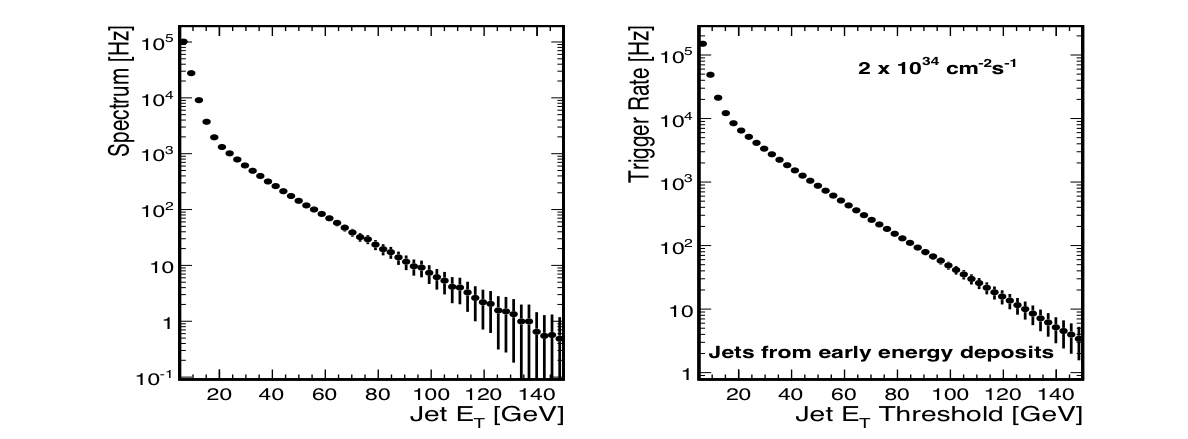
\includegraphics[scale=0.8]{plots/hcaltdr_plot.png}}
\caption{The spectrum of fake jets in HF induced by early jet candidates at Level-1, for an instantaneous luminosity of $2 \times 10^{34} \textrm{cm}^{-1} \textrm{s}^{-1}$.}
\label{fig:hcaltdr_plot}
\end{figure}
\vspace{5mm}

\section{Framework and datasets}
\label{sec:tech}

The performance of the L1 calorimeter trigger has been primarily evaluated with datasets collected using zero- or minimum-bias triggers~\cite{2012note}. However these provide adequate statistical precision only for performance evaluation of calorimeter triggers with low energy thresholds. For higher energy thresholds, such event samples become insufficient to study trigger performance and events collected using a single muon trigger are used instead. This procedure has been shown to be unbiased for the triggers under study.

In this note, events from the single muon dataset were used to evaluate the performance at high energies:

\texttt{/SingleMu/Run2012D-PromptReco-v1/AOD}

The sample was further selected by filtering events based on isolated muon triggers (\texttt{HLT\_IsoMu}).

To cross-check the performance results with the ones presented in Fig.~\ref{fig:hcaltdr_plot}, the analysis was also repeated using events from the minimum bias datasets:

\texttt{/MinimumBias/Run2012D-PromptReco-v1/AOD}

where events were further selected based on zero bias triggers (\texttt{HLT\_ZeroBias}).

In both cases, the analysis used only events certified with the Golden JSON file:

\texttt{Cert\_190456-208686\_8TeV\_PromptReco\_Collisions12\_JSON.txt}.

The events from the 2012 datasets above were analysed within the official L1Ntuple framework~\cite{l1ntpl}. The L1 jet collections were accessed using standard \texttt{l1Extra} candidates from the nominal and previous bunch crossing.

\section{Level-1 jet triggers}
\label{sec:l1jetalgo}

The jet finding algorithm in the L1 trigger searches for local maxima in calorimeter region ($\Delta \eta \times \Delta \phi =
0.348 \times 0.348$) \et and then sums the $3\times3$ block of trigger regions around the maximum \et region (see
Fig.~\ref{fig:l1jetalgo}). The central maximum trigger region is required to have more energy than the surrounding
regions, and also be higher than a threshold, the latter to suppress pile-up. After jets are found, a programmable $\eta$ and \pt dependent jet energy scale correction is applied.

Jets with $|\eta|>3.0$ are classified as forward jets, whereas those with $|\eta|<3.0$ are classified as central or $\tau$ jets, 
depending on extra isolation and pattern-recognition criteria. The four highest energy central, forward and $\tau$ jets are used to make the CMS L1 trigger decision and are used in the study presented in this note.

\begin{figure}[h!]
\centering
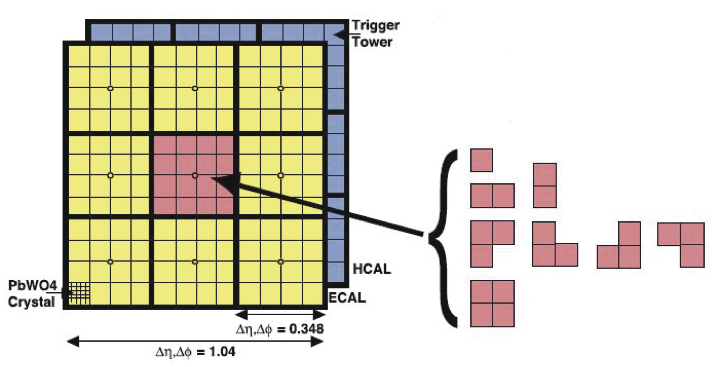
\includegraphics[scale=1.0]{plots/L1JetAlgorithm.png}
\caption{Illustration of the Level-1 jet finding algorithm.}
\label{fig:l1jetalgo}
\end{figure}
\vspace{5mm}

\section{Trigger pre-firing rates}

No pre-firing effects are expected or have been observed in ECAL so we assume any observed effects result from the hadronic calorimeter (HCAL). A measure of the pre-firing effect from L1 jet triggers in the barrel-endcap (HB/HE) and forward (HF) regions of the hadronic calorimeter, is evaluated by calculating the relative rate of jet triggers coming from early energy deposits in the calorimeters (BX=-1), with respect to the number of Jet triggers firing in the nominal collision (BX=0). 

In the next two sections, the relative rate of L1 jet pre-firing is determined, as a function of the L1 jet threshold, for the HB/HE and HF regions separately.

\subsection{Pre-firing rates in HB/HE}
\label{sec:rates_hbhe}

The pre-firing rate of L1 jets in the HB/HE region is estimated as a function of the L1jet \pt threshold. Only the leading L1 jet candidate from each of BX=-1, 0 is used, as this is equivalent to a L1 jet trigger firing. The L1 jet \pt spectrum is shown for Jets firing in the nominal (BX=0) and jets from early energy deposits appearing in BX=-1, for minimum bias events (see Fig.~\ref{fig:l1jetpt_minb}) and single muon events (see Fig.~\ref{fig:l1jetpt_smu}). We note that the peak at the $\pt=250$ \GeV bin of the distributions corresponds to L1 jet candidates with saturated \et. 

To calculate the relative rate of events prefiring in the HB/HE region, we first integrate the distributions over the jet \pt spectrum, and extract a rate of events firing at BX=0 (black distributions) and a rate of events with L1 jets pre-firing at BX=-1 (red distributions). This is shown as a function of the L1jet \pt threshold in both the minumum bias (Fig.~\ref{fig:hbherate_minb}) and single muon (Fig.~\ref{fig:hbherate_smu}) events. The rate is shown in arbitrary units. The ratio of the two distributions, namely the ratio between BX=-1 and BX=0 rates, gives a measure of the relative rate of prefiring.

\begin{2figures}{h!}
\centering
\resizebox{1.\linewidth}{0.45\height}{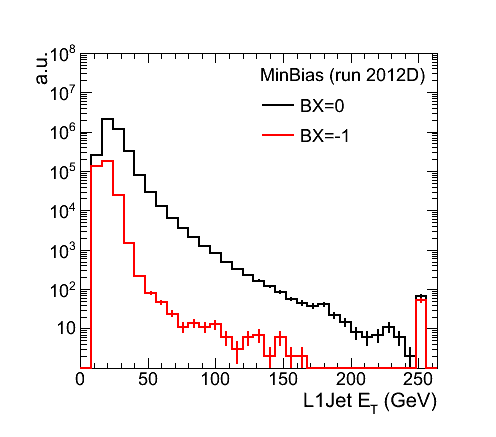
\includegraphics{plots/ptSpectrum_cenJets_MinBias_runD.png}} &
\resizebox{1.\linewidth}{0.45\height}{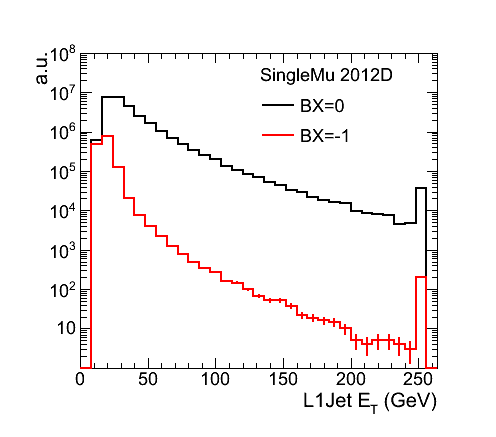
\includegraphics{plots/ptSpectrum_cenJets_SingleMu_runD.png}} \\
\caption{Level-1 jet \pt spectrum for nominal (black) and early (red) candidates in zero-bias triggered events.}\label{fig:l1jetpt_minb}  &
\caption{Level-1 jet \pt spectrum for nominal (black) and early (red) candidates in single muon triggered events.}\label{fig:l1jetpt_smu}
\end{2figures}
\begin{2figures}{h!}
\centering
\resizebox{1.\linewidth}{0.45\height}{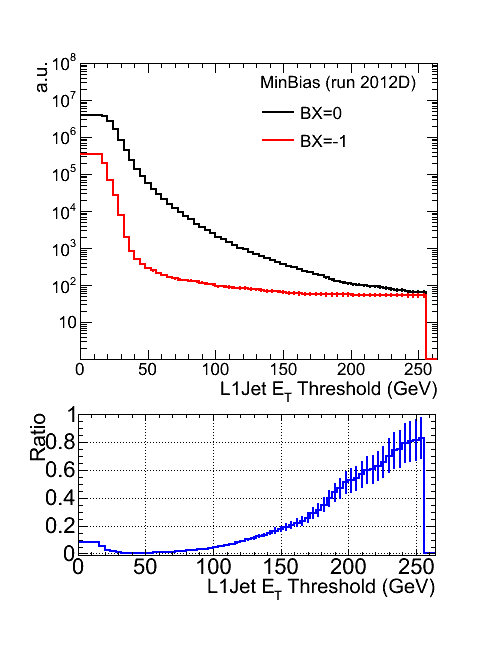
\includegraphics{plots/Rate_cenJets_MinBias_runD.png}} &
\resizebox{1.\linewidth}{0.45\height}{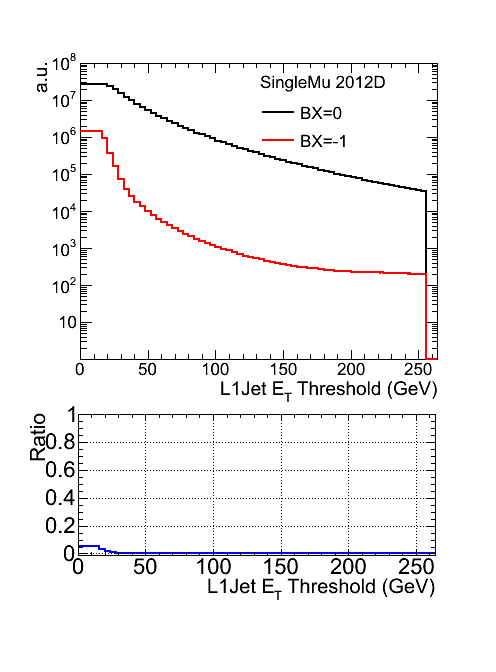
\includegraphics{plots/Rate_cenJets_SingleMu_runD.png}} \\
\caption{Level-1 Jet rate for nominal (black) and early (red) candidates in zero-bias triggered  events.}\label{fig:hbherate_minb} &
\caption{Level-1 Jet rate for nominal (black) and early (red) candidates in single muon triggered events.}\label{fig:hbherate_smu}
\end{2figures}

It is noted that the relative rates of early triggers show strikingly different behaviour for minimum bias and single muon events. This can be explained in Figs.~\ref{fig:l1jetpt_minb} and~\ref{fig:l1jetpt_smu}, where the peak in the overflow bin of the L1 jet spectrum in mimimum bias events is approximately the same size between L1 jets at BX=-1 and jets at BX=0. This is in contrast with the single muon events, where the relative amount of jet triggers between BX=-1 and BX=0 stays constant beyond a certain L1 jet threshold.

The unexpectedly large peak in the overflow bin for the early L1 jet candidates in minimum bias events is thought to be noise. To establish this, only the events with L1 jets of saturated \et were investigated. The $\eta$ and $\phi$ distributions for out of time L1 jets of saturated \et and for in time L1 jets of saturated \et can be seen in Figs.~\ref{fig:early_eta_phi} and~\ref{fig:central_eta_phi}, respectively. As can be seen, out of time L1 jets of saturated \et come predominantly from suspicious spikes in $\eta/\phi$, which is an observation consistent with noise. This effect seems to be irreducible at L1.

We conclude that for the single muon triggered sample, where the noise is less prevalent, the rate of pre-firing is at a neglible level.

% Early L1jets with saturated Et in MinBias events
\begin{figure}
\centering
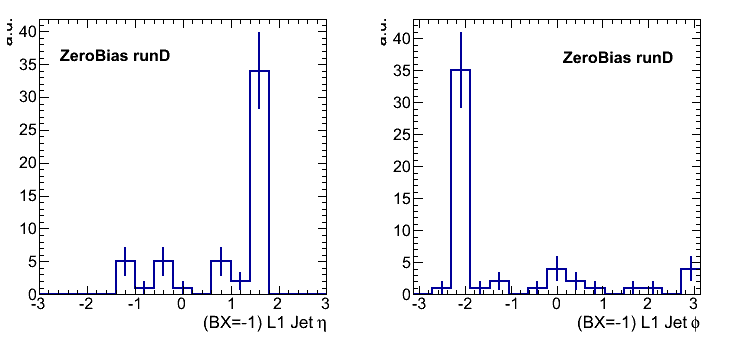
\includegraphics[scale=0.5]{plots/early_l1Jet_withSaturatedEt_eta_phi_ZeroBias_runD.png}
\caption{L1 jet $\eta$ (left) and $\phi$ (right) distributions for candidates with saturated \et in the early BX=-1 bunch crossing in minimum bias triggered events.}
\label{fig:early_eta_phi} 
\end{figure}
\begin{figure}
\centering
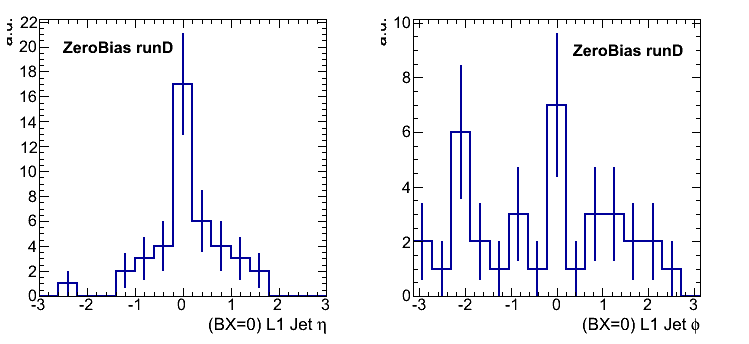
\includegraphics[scale=0.5]{plots/central_l1Jet_withSaturatedEt_eta_phi_ZeroBias_runD.png}
\caption{L1 jet $\eta$ (left) and $\phi$ (right) for candidates with saturated \et in the nominal BX=0 bunch crossing in minimum bias triggered events.} 
\label{fig:central_eta_phi} 
\end{figure}

\subsection{Pre-firing rates in HF}
\label{sec:rates_hf}

The relative pre-firing rate is also evaluated for L1 jets in the HF. As in the previous section, the L1 jet \pt spectrum is shown for jets at BX=0 (in black) and BX=-1 (in red), both for minimum bias events (see Fig.~\ref{fig:fwdjetpt_minb}) and single muon events (see Fig.~\ref{fig:fwdjetpt_smu}). In this case, the effect from the overflow bin in the distributions (jets with saturated \pt), gives rise to a plateau behaviour in the relative rate of pre-firing in a similar way between minimum bias and single muon events (Figs.~\ref{fig:fwdrate_minb} and~\ref{fig:fwdrate_smu}). The rate of pre-firing is significant in both samples.

\begin{2figures}{h!}
\centering
\resizebox{1.\linewidth}{0.45\height}{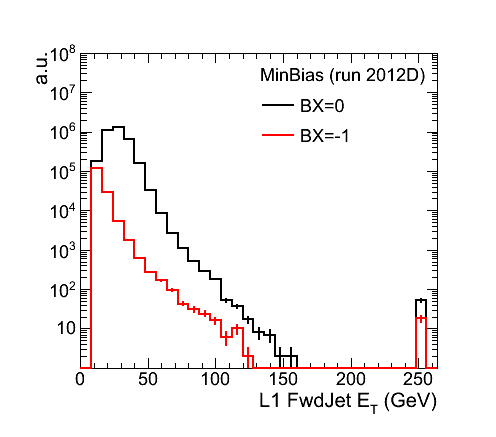
\includegraphics{plots/ptSpectrum_FwdJets_MinBias_runD.png}} &
\resizebox{1.\linewidth}{0.45\height}{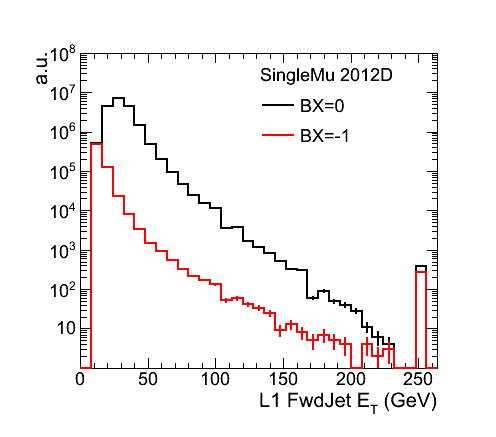
\includegraphics{plots/ptSpectrum_FwdJets_SingleMu_runD.png}} \\
\caption{Level-1 Jet spectrum in the HF, for nominal (black) and early (red) candidates in zero bias triggered events.}\label{fig:fwdjetpt_minb} &
\caption{Level-1 Jet spectrum in the HF, for nominal (black) and early (red) candidates in single muon triggered events.}\label{fig:fwdjetpt_smu}
\end{2figures}
\begin{2figures}{h!}
\centering
\resizebox{1.\linewidth}{0.45\height}{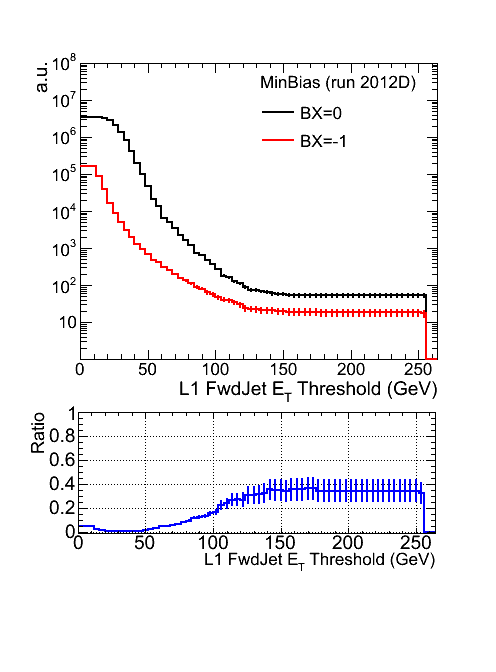
\includegraphics{plots/Rate_FwdJets_MinBias_runD.png}} &
\resizebox{1.\linewidth}{0.45\height}{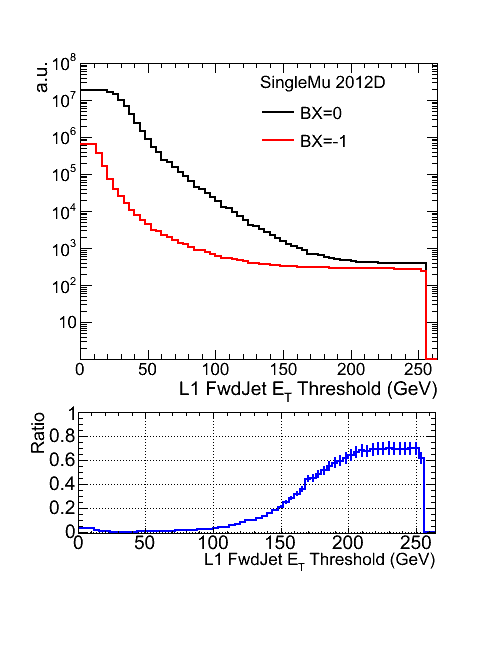
\includegraphics{plots/Rate_FwdJets_SingleMu_runD.png}} \\
\caption{Level-1 Jet rate in the HF, for nominal (black) and early (red) candidates in zero bias' triggered events.}\label{fig:fwdrate_minb} &
\caption{Level-1 Jet rate in the HF, for nominal (black) and early (red) candidates in single muon triggered events.}\label{fig:fwdrate_smu}
\end{2figures}

\section{Impact of upgraded HF PMTs}

The difference in pre-firing between the old and new PMTs in the HF in the 2012 data was investigated (as in the HCAL TDR~\cite{hcaltdr}). From a private communication~\cite{privcomm}, a full list of ($i\eta, i\phi$) regions for the new PMTs is shown in Fig.~\ref{fig:newpmts}, which corresponds to $i \phi=43$ in the negative $\eta$ HF detector. The same figure shows the new PMTs location in a L1 jet ($i\eta, i\phi$) map. The new PMTs are expected to reduce the rate of pre-firing by a factor of 2 to 5.

With this information, it is possible to test what to expect in 2015 running. The area of a L1 jet is much larger than the area of new PMTs installed, so the improvement from the new PMTs will be diluted. Therefore the measurement may be considered a lower limit on the improvement. The single muon dataset was used and compared the pre-firing rate for L1 jets centred on region of the new PMTs ($i \phi=43$ negative $\eta$) versus the rate in the region of other PMTs ($i \phi=39$ negative $\eta$ was used). This is shown in Figs.~\ref{fig:oldpmts} and~\ref{fig:newpmts}, respectively.

A direct comparison is given by the ratio of the pre-firing rates as shown in Fig.~\ref{fig:imp}, indicating a lower limit on the expected improvement of a reduction factor of $3-4$ for jet \pt thresholds greater than 100\GeV, compatible with expectations for the new PMTs.

\begin{figure}
\centering
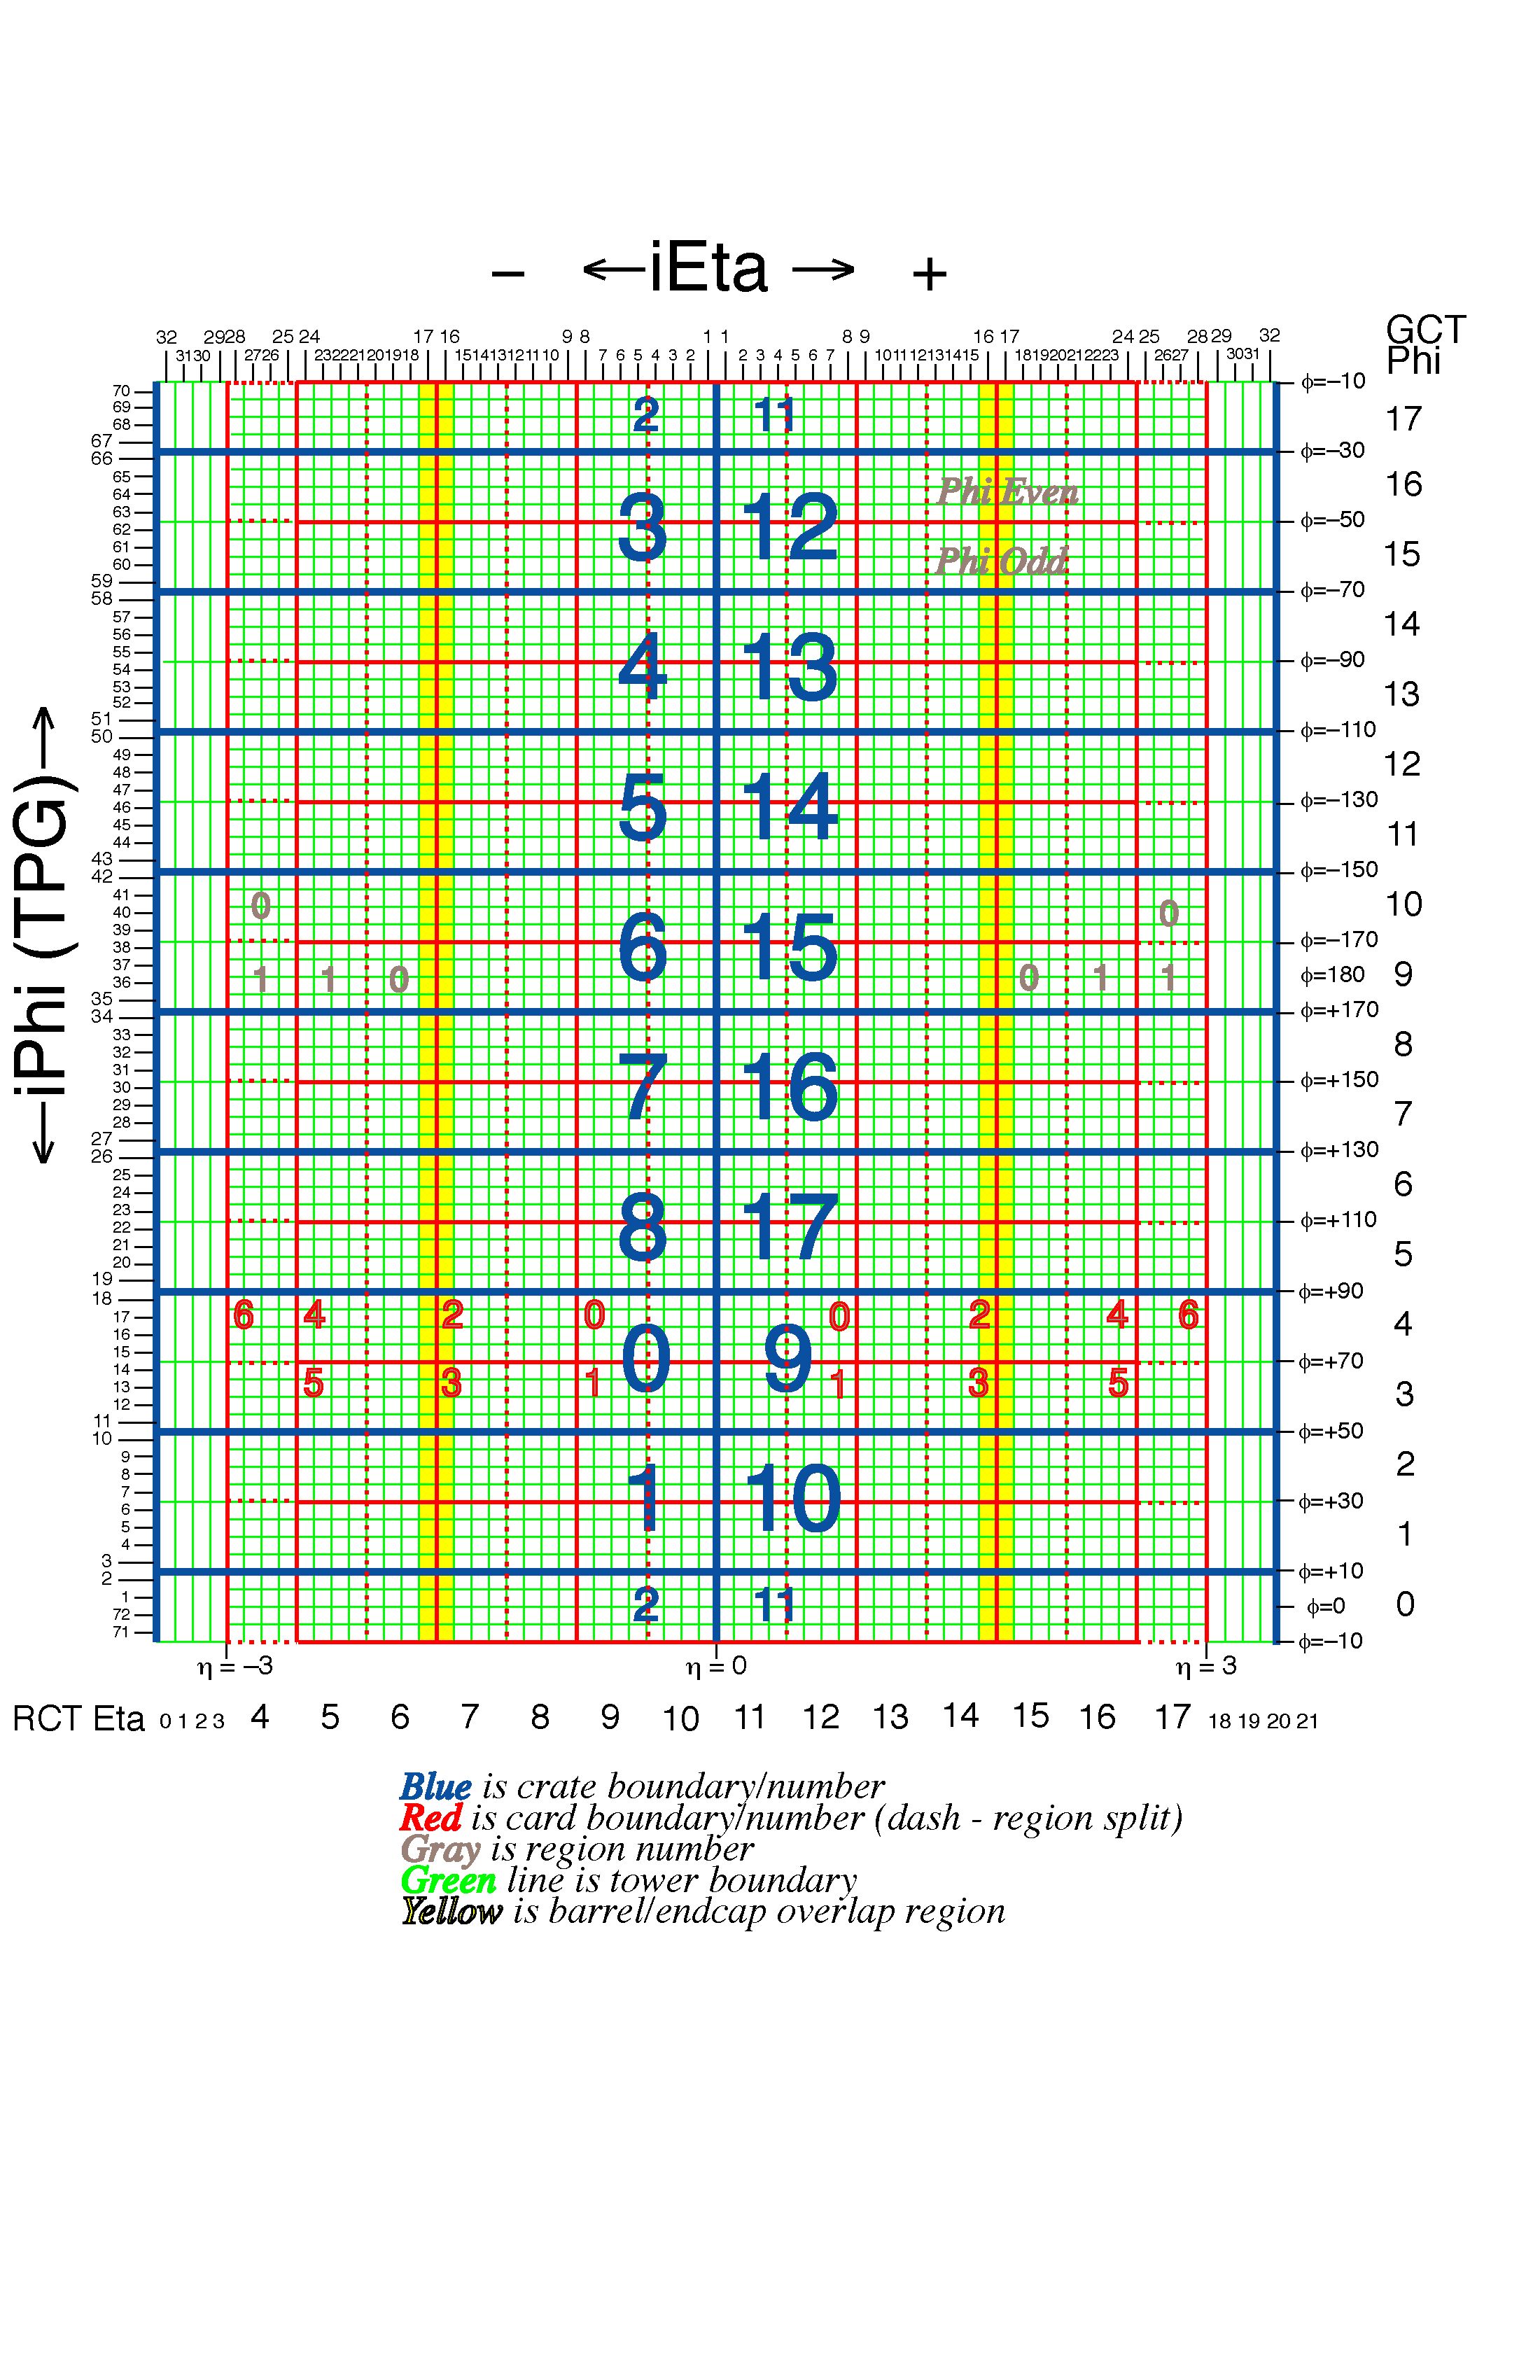
\includegraphics[scale=0.23]{plots/towers_ieta_iphi_2009.png}
\caption{Regional calorimeter trigge map in trigger tower space.} 
\end{figure}
\vspace{5mm}

\begin{figure}
\centering
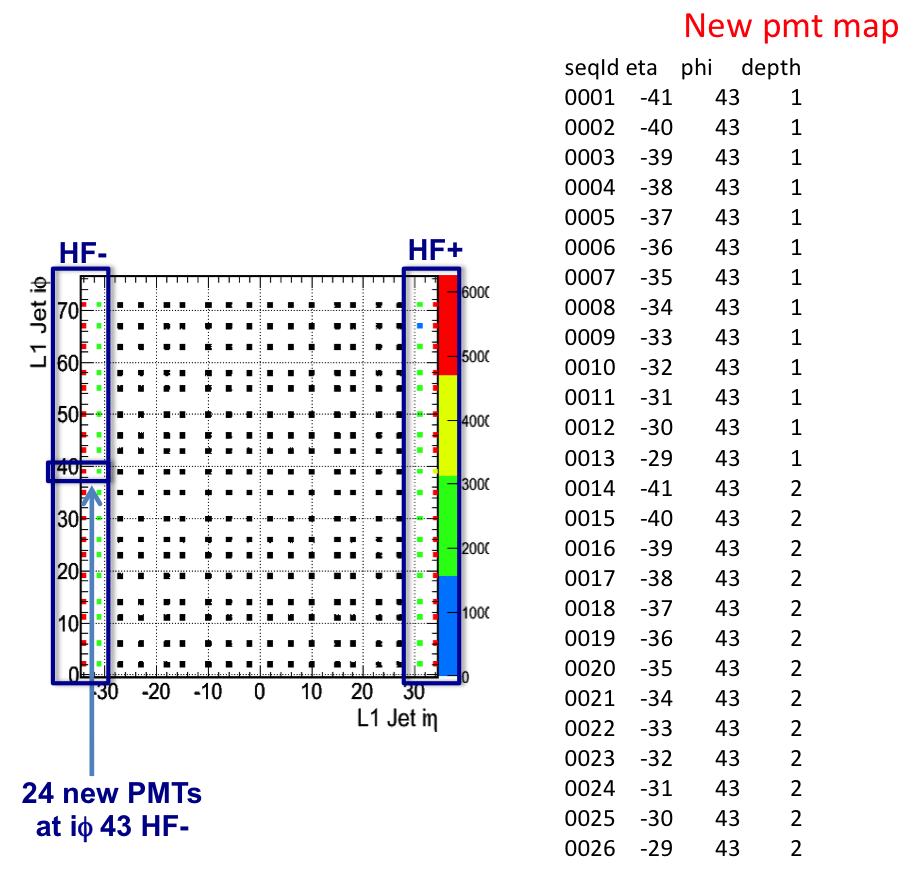
\includegraphics[scale=0.7]{plots/upgradedPMTs_regions_in2012.png}
%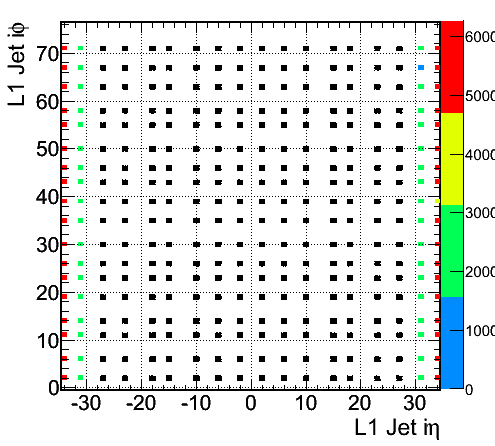
\includegraphics[scale=0.5]{plots/l1Jet_ieta_iphi_BX0_fullmap.png}
\caption{L1 jet ($\eta$,$\phi$) mapped to ($i \eta$, $i \phi$) tower ID. Black dots correspond to L1 jets falling into the HB/HE regions, whereas coloured dots correspond the L1 jets in the HF ($| i \eta| > 28$). The regions where the upgraded PMTs were installed during 2012 data is shown superimposed at $i \phi=43$ and negative $\eta$. }
\label{fig:newpmts} 
\end{figure}
 
\begin{2figures}{h!}
\centering
\resizebox{1.\linewidth}{0.45\height}{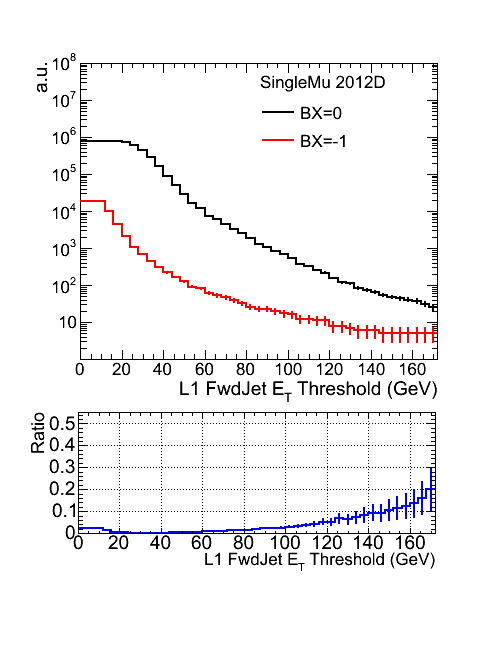
\includegraphics{plots/oldPMTs_Rate_FwdJets_SingleMu_runD.png}} &
\resizebox{1.\linewidth}{0.45\height}{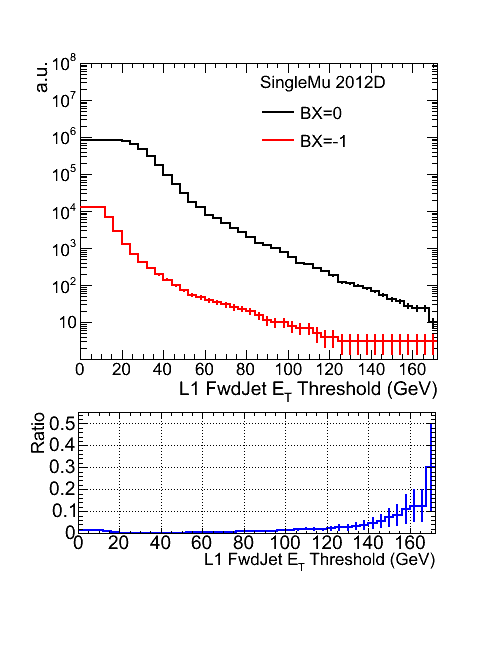
\includegraphics{plots/upgradedPMTs_Rate_FwdJets_SingleMu_runD.png}} \\
\caption{L1 jet rate in the HF, for nominal (black) and early (red) candidates in single muon triggered events. L1 jets fall into regions with $i \phi=39$ HF- (old PMTs region).}\label{fig:oldpmts} &
\caption{L1 jet rate in the HF, for nominal (black) and early (red) candidates in single muon' triggered events. L1 jets fall into regions with $i \phi=43$ HF- (regions with upgraded PMTs).}\label{fig:newpmts}
\end{2figures}
\begin{figure}
\centering
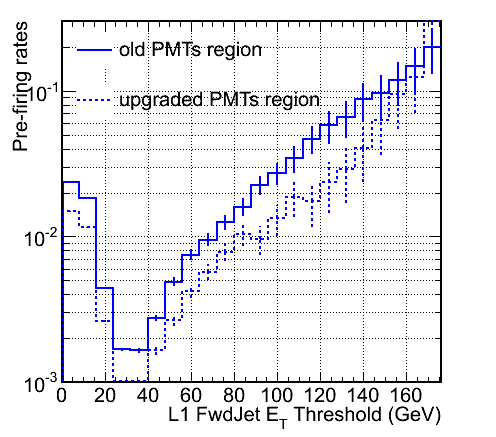
\includegraphics[scale=0.45]{plots/rates_comparison_old-vs-new-PMTs.png}
\caption{Pre-firing rates comparison for L1 jets falling into $i \phi=39$ negtive $\eta$ (old PMTs region) shown in solid blue, and $i \phi=43$ negative $\eta$ (i.e. regions with upgraded PMTs) shown in dashed blue. }
\label{fig:imp} 
\end{figure}

\section{Performance with physics skims}

Finally, the effect of pre-firing on some physics skims provided by the Trigger Studies Group (TSG)~\cite{tsg} was evaluated. The physics samples used for this analysis include events with W/Z decaying to leptons, $t \bar{t}$ events, $H \rightarrow WW$ as well as $H \rightarrow \tau\tau$ events. All events come from 2012 datasets, based on some pre-defined trigger paths which enchance the fraction of signal events.

Figures~\ref{fig:p1_hbhe},~\ref{fig:p2_hbhe},~\ref{fig:p3_hbhe} and~\ref{fig:p4_hbhe} show the prefiring rates in HB/HE, whereas Figs.~\ref{fig:p1_hf},~\ref{fig:p2_hf},~\ref{fig:p3_hf} and~\ref{fig:p4_hf} show the prefiring rates in HF. The effect of pre-firing is negligible for these physics samples.

\begin{2figures}{h!}
\centering
\resizebox{1.\linewidth}{0.45\height}{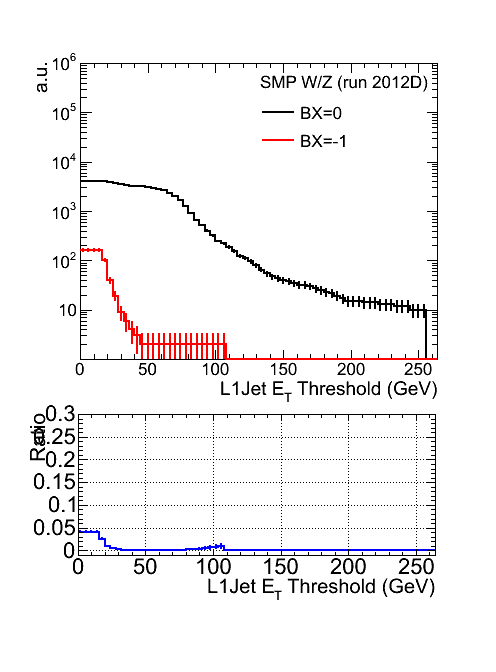
\includegraphics{plots/l1Jet_rate_HBHE_SMP_WZ_TSGskim.png}} &
\resizebox{1.\linewidth}{0.45\height}{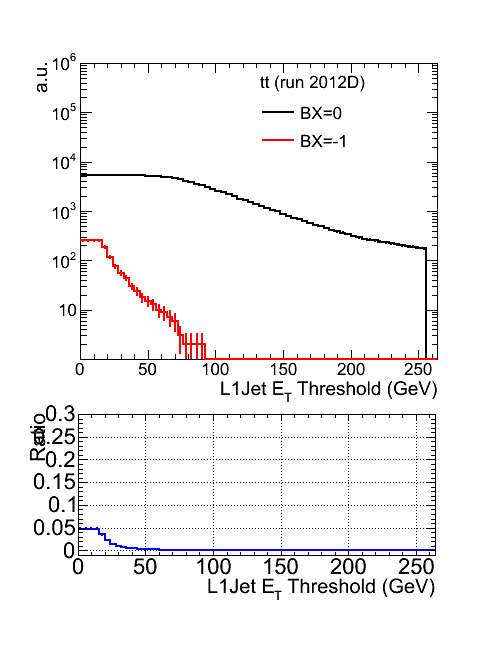
\includegraphics{plots/l1Jet_rate_HBHE_tt_TSGskim.png}} \\
\caption{Level-1 Jet rate for nominal (black) and early (red) candidates in $W/Z \rightarrow$ leptons events, for HB/HE regions.}\label{fig:p1_hbhe} &
\caption{Level-1 Jet rate for nominal (black) and early (red) candidates in $t \bar{t}$ events, for HB/HE regions.}\label{fig:p2_hbhe}
\end{2figures}
\begin{2figures}{h!}
\centering
\resizebox{1.\linewidth}{0.45\height}{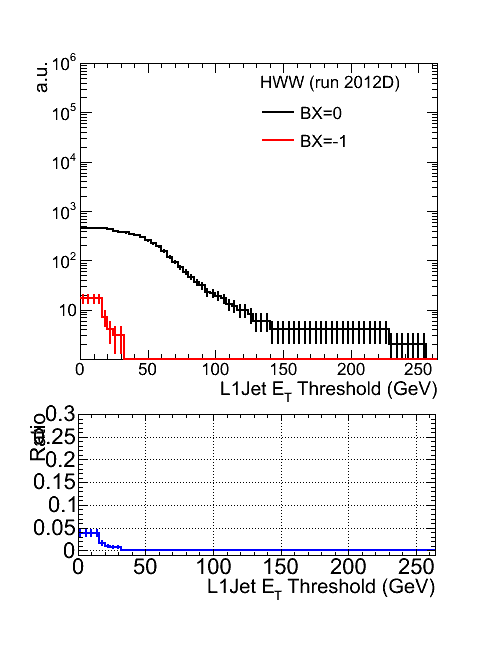
\includegraphics{plots/l1Jet_rate_HBHE_HWW_TSGskim.png}} &
\resizebox{1.\linewidth}{0.45\height}{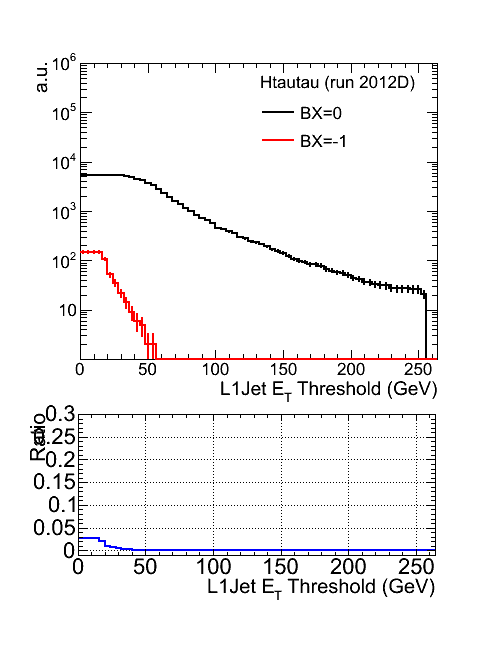
\includegraphics{plots/l1Jet_rate_HBHE_Htautau_TSGskim.png}} \\
\caption{Level-1 Jet rate for nominal (black) and early (red) candidates in $ H \rightarrow WW$ events, for HB/HE regions.}\label{fig:p3_hbhe} &
\caption{Level-1 Jet rate for nominal (black) and early (red) candidates in $ H \rightarrow \tau \tau$ events, for HB/HE regions.}\label{fig:p4_hbhe}
\end{2figures}

% TSG skims at HF
\begin{2figures}{h!}
\centering
\resizebox{1.\linewidth}{0.45\height}{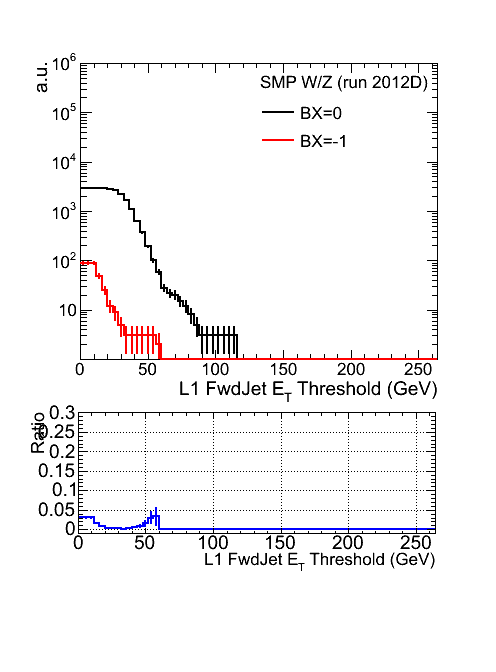
\includegraphics{plots/l1Jet_rate_HF_SMP_WZ_TSGskim.png}} &
\resizebox{1.\linewidth}{0.45\height}{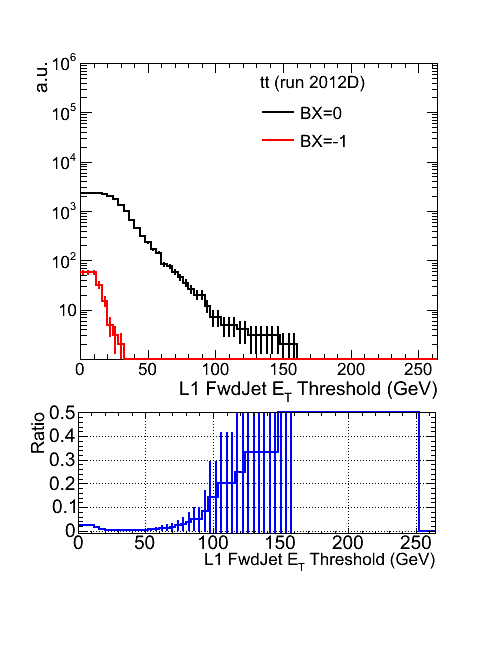
\includegraphics{plots/l1Jet_rate_HF_tt_TSGskim.png}} \\
\caption{Level-1 Jet rate for nominal (black) and early (red) candidates in $W/Z \rightarrow$ leptons events, in the HF region.}\label{fig:p1_hf} &
\caption{Level-1 Jet rate for nominal (black) and early (red) candidates in $t \bar{t}$ events, in the HF region.}\label{fig:p2_hf}
\end{2figures}
\begin{2figures}{h!}
\centering
\resizebox{1.\linewidth}{0.45\height}{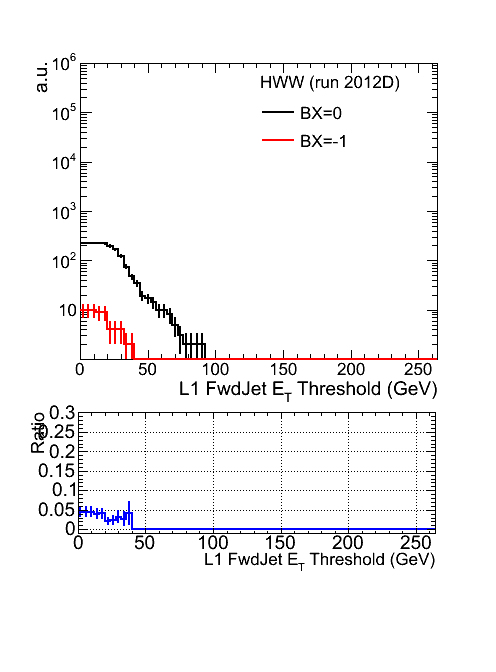
\includegraphics{plots/l1Jet_rate_HF_HWW_TSGskim.png}} &
\resizebox{1.\linewidth}{0.45\height}{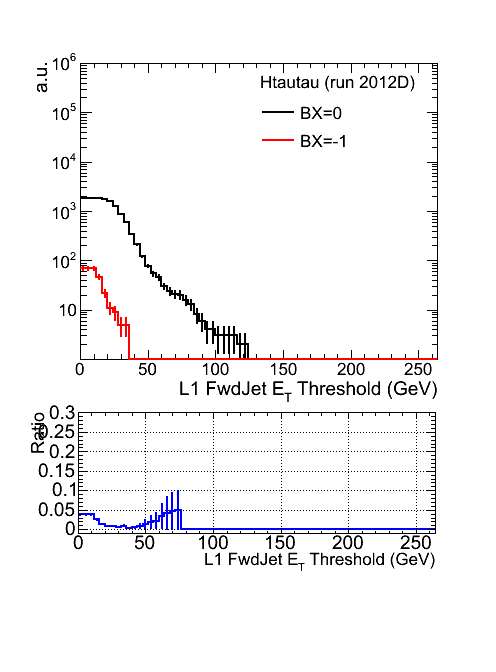
\includegraphics{plots/l1Jet_rate_HF_Htautau_TSGskim.png}} \\
\caption{Level-1 Jet rate for nominal (black) and early (red) candidates in $ H \rightarrow WW$ events, in the HF region.}\label{fig:p3_hf}  &
\caption{Level-1 Jet rate for nominal (black) and early (red) candidates in $ H \rightarrow \tau \tau$ events, in the HF region.}\label{fig:p4_hf} 
\end{2figures}

\section{Conclusions}

The studies presented in this note show that pre-firing is not expected to be a significant effect in HB/HE in 25~ns running. The relative rate of pre-firing in HF under 2012 conditions has been determined. It was not possible to draw any strong conclusions from the small area of HF which was already instrumented with new PMTs in 2012, however the reduction in pre-firing rate appears to be consistent with expectation. The procedure to measure the rate of pre-firing has been established and a measurement with the 50~ns data in 2015 will determine how the L1 trigger should run in 25~ns conditions in 2015.

\newpage
%% **DO NOT REMOVE BIBLIOGRAPHY**
\bibliography{auto_generated}   % will be created by the tdr script.

\begin{thebibliography}{99}

\bibitem{hcaltdr} ``CMS Technical Design Report for the Phase I Upgrade of the Hadron Calorimeter'', CMS-TDR-010, CERN-LHCC-2012-015.
\bibitem{2012note} ``Performance of the Level-1 Trigger for Jets and Energy Sums in 2012'', CMS AN-2013/370 (2013).
\bibitem{l1ntpl} https://twiki.cern.ch/twiki/bin/viewauth/CMS/L1TriggerDPGNtupleProduction
\bibitem{privcomm} S.~Kunori et. al., Private Communication, October 2014.
\bibitem{tsg} https://twiki.cern.ch/twiki/bin/viewauth/CMS/HLTDataSkimsForValidation

\end{thebibliography}

%% examples of appendices. **DO NOT PUT \end{document} at the end
\clearpage
\appendix

\end{document}


